%!TEX program = xelatex
\documentclass[aspectratio=169]{beamer}

\usepackage{blindtext}

\usetheme{Execushares}

\title{Structured Sparsity in\\Numerical Optimisation}
\subtitle{Universit\'{e} C\^ote D'Azur, Inria, France}
\author{Matteo Frigo}
\date{Nice - December 4, 2017}

\usepackage{amsmath,amssymb,amsfonts,amsthm}
\usepackage{graphicx}
\usepackage{pgf,tikz}
\usetikzlibrary{arrows}
\definecolor{qqzzqq}{rgb}{0.,0.6,0.}
\definecolor{ffqqqq}{rgb}{1.,0.,0.}
\definecolor{qqqqff}{rgb}{0.,0.,1.}
\definecolor{mygreen}{rgb}{0.0, 0.5, 0.0}
\usepackage{wasysym}

%\theoremstyle{definition}
%\newtheorem{problem}{Problem}
%\newtheorem{definition}{Definition}
%\newtheorem{eg}{Example}
%
%\theoremstyle{plain} 
%\newtheorem{theorem}{Theorem}
%\newtheorem{proposition}{Proposition}
%\newtheorem{lemma}{Lemma}
%\newtheorem{property}{Property}
%\newtheorem{corollary}{Corollary}
%\newtheorem{algo}{Algorithm}

\DeclareMathOperator{\Prox}{prox}
\newcommand{\prox}[2]{\Prox_{#1}\left({#2}\right)}

\newcommand{\HH}{\mathcal{H}}
\newcommand{\NN}{\mathbb{N}}
\newcommand{\ZZ}{\mathbb{Z}}
\newcommand{\QQ}{\mathbb{Q}}
\newcommand{\RR}{\mathbb{R}}
\newcommand{\rd}{\mathbb{R}^d}
\newcommand{\rn}{\mathbb{R}^n}
\newcommand{\CC}{\mathbb{C}}
\newcommand{\norm}[1]{\left\|#1\right\|}
\newcommand{\normtwosq}[1]{\left\|#1\right\|_2^2}
\newcommand{\onehalf}{\frac{1}{2}}
\newcommand {\matlab} {$\text{Matlab}^{\circledR}$\,}
\newcommand {\expect} {\mathbb{E}}
\newcommand {\prob} {\mathbb{P}}
\renewcommand{\epsilon}{\varepsilon}
%\renewcommand{\theta}{\vartheta}
%\renewcommand{\rho}{\varrho}
\renewcommand{\phi}{\varphi}
\hyphenation{sub-dif-fe-ren-tial}
\hyphenation{COMMIT}

\DeclareMathOperator*{\argmin}{argmin}
\DeclareMathOperator{\dom}{dom}

\setcounter{showProgressBar}{0}
\begin{document}

	\frame{\titlepage}
	
	\begin{frame}
	\frametitle{Matteo Frigo}
	\begin{minipage}{.45\textwidth}
	\begin{center}
	
\includegraphics[height=1cm,keepaspectratio]{img/logo_inria}\\ \quad \\
	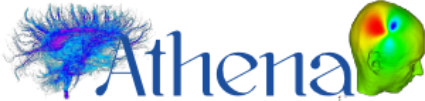
\includegraphics[height=1cm,keepaspectratio]{img/athena-logo}\\ \quad \\
	
\includegraphics[height=1cm,keepaspectratio]{img/flag_yellow_high}\qquad
	
\includegraphics[height=1cm,keepaspectratio]{img/erc_logo}
	\end{center}
	\end{minipage}
	\quad
	\begin{minipage}{.45\textwidth}
	\begin{itemize}
	\item PhD Student @ EDSTIC
	\item Supervisor: Rachid Deriche
	\item Inria - Athena Project Team
	\item ERC Computational Brain Connectivity Mapping 
	\end{itemize}
	\end{minipage}
	\end{frame}
	
	\begin{frame}
		\frametitle{Contents}
		\begin{enumerate}
			\item Mathematics \\ \textcolor{ExecusharesGrey}{\footnotesize\hspace{1em} Proximal Operator, FISTA, convex proper lower semi continuous}
			\item Regularisation theory  \\ \textcolor{ExecusharesGrey}{\footnotesize\hspace{1em} Sparsity, Hierarchy, Lasso}
			\item Brain Imaging \\ \textcolor{ExecusharesGrey}{\footnotesize\hspace{1em} Tractography, dMRI, Connectomics}
		\end{enumerate}
	\end{frame}
	
	
	\section{Mathematics}
		\setcounter{showSlideNumbers}{1}
		\begin{frame}
			\frametitle{Numerical Optimisation}
			\quad \\
			\begin{itemize}
			\item $\HH$ is a set
			\item $\Phi: \HH\to\RR$
			\item Find \begin{equation}\nonumber x^* = \argmin_{x\in\HH}\Phi(x)\end{equation}
			\end{itemize}
			
			\pause
			\vfill
			
			Our setting:
			\begin{itemize}
			\item $\HH=\rd$
			\item $\Phi(x) := f(x) + g(x)$
				\begin{itemize}
				\item $f(x)$ is convex and has $L$-Lipschitz continuous gradient
				\item $g(x)$ is convex and lower semi-continuous
				\end{itemize}
			\item Find \begin{equation}\nonumber x^* = \argmin_{x\in\rd}f(x)+g(x)\end{equation}
			\end{itemize}
			
		\end{frame}

		\begin{frame}
			\frametitle{Smooth case}
			\begin{minipage}{.45\textwidth}
			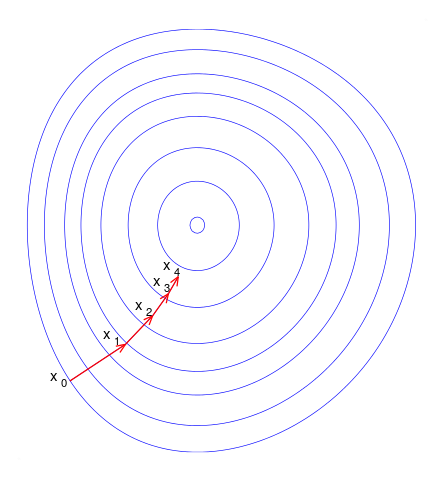
\includegraphics[width=\textwidth]{img/gradientdescent}
			\end{minipage}\qquad
			\begin{minipage}{.45\textwidth}
			Smooth case:
			\begin{equation}\nonumber
			x^*=\argmin_{x\in\rd}f(x).
			\end{equation}
			Iteration:
			\begin{equation}
			\nonumber
			x^+ = x - \gamma\nabla f(x)
			\end{equation}
			with $\gamma=\frac{1}{L}$
			\end{minipage}
		\end{frame}

		\begin{frame}
		\frametitle{Non-smooth case}
		Let $\{C_j\}_j$ sequence of cvx subsets of $\rd$ with non-empty intersection,
		\begin{equation}
		\nonumber
		x^*=\argmin_{x\in \rd}\sum_j \iota_{C_j}(c)
		\end{equation}
		\pause
		POCS: Projection Onto Convex Sets
		\begin{equation}
		\nonumber
		x_{k+1} = \Pi_{C_1}\Pi_{C_2}\cdots\Pi_{C_N} x_k.
		\end{equation}
		\pause
		Each projection is the solution of 
		\begin{equation}
		\nonumber
		\argmin_{y\in \rd}\frac{1}{2}\normtwosq{x_k-y} + \iota_{C_j}(y).
		\end{equation}
		\end{frame}
		
		\begin{frame}
		\frametitle{Proximal operator}
		$\Gamma_0(\mathcal{H}) = \left\{g:\mathcal{H}\to\RR\text{ l.s.c. and cvx with } \dom(g)\ne\emptyset\right\}$
		\quad \\ \quad \\
		\begin{definition}[Proximal Operator]
		Let $g\in\Gamma_0(\RR^N)$. For every $x \in \RR^N$, the minimisation problem
		\begin{equation}
		\nonumber
		\argmin_{y\in\RR^N} g(y) + \frac{1}{2}\normtwosq{x-y}
		\end{equation}
		admits a unique solution called $\prox{g}{x}$.
		\end{definition}
		\end{frame}

		\begin{frame}
		\frametitle{Properties of $\Prox$}
		Separability:
		\begin{equation}
		\nonumber g(x,y) = \phi(x)+\psi(y) = \prox{\phi}{x} + \prox{\psi}{y}
		\end{equation}
		
		{Nonexpansiveness}:
		\begin{equation}
		\nonumber \normtwosq{\prox{g}{x}-\prox{g}{y}} \le \left(x-y\right)^T\left(\prox{g}{x} - \prox{g}{y}\right)
		\end{equation}
		
		Resolvent operator: 
		\begin{equation}
		\nonumber \prox{g}{\cdot} = \left(I + \partial g\right)^{-1} (\cdot)
		\end{equation}
		\end{frame}
		
		\begin{frame}
		\frametitle{Properties of $\Prox$: part 2}
		\begin{definition}
		The convex conjugate of $g:X\to\RR$ is $g^*:X^*\to\RR$
		\begin{equation}
		\nonumber
		g^*(\xi) = \sup_{x\in X}\left\{\left<\xi,x\right>-g(x)\right\}.
		\end{equation}
		\end{definition}		
		\pause
		{Moreau decomposition}:
		\begin{gather}
		\nonumber v = \prox{g}{v} + \prox{g^*}{v}\\
		\nonumber v = \Pi_L(v) + \Pi_{L^\perp}(v)\\
		\nonumber v = \Pi_K(v) + \Pi_{K^\circ}(v)
		\end{gather}
		\begin{proof}
		$2+2=4-1=3$ quick mafhs.
		\end{proof}
		\end{frame}
		

		
		\begin{frame}
		\frametitle{Key property}
		\begin{center}
		A point $x^*\in \RR^n$ is a minimiser of $g$ if and only if 
		\end{center}
		\begin{equation}
		\nonumber \prox{g}{x^*} = x^*.
		\end{equation}
		\end{frame}
		
		\begin{frame}
		\frametitle{Greedy algorithm for non-smooth optimisation}
		\begin{equation}
		\nonumber x^* = \argmin_{x\in \rd} g(x)
		\end{equation}
		\pause
		Considerations:
		\begin{itemize}
		\pause\item $\Prox$ is non-expansive
		\pause\item The minimiser $x^*$ is a fixed point of $\Prox$
		\end{itemize}
		\pause
		Iteration:
		\begin{equation}\nonumber
		x_{k+1} = \prox{g}{x_k}
		\end{equation}
		
		\pause
		If we don't know anything about the Lipschitz constant of $\Prox_g$
		\begin{equation}
		\nonumber x_{k+1} = [(1-\alpha)I + \alpha\Prox_g](x_k)
		\end{equation}
		\quad \\
		\begin{center}
		\textcolor{ExecusharesGrey}{\tiny Cominetti et al., On the rate of convergence of Krasnoselskii-Mann iterations and their connection with sums of Bernoullis, 2014}
		\end{center}
		\end{frame}
		
%		\begin{frame}
%		\frametitle{Interpretation}
%		Gradient descent of the Moreau envelope
%		\begin{equation}
%		\nonumber M_{f} = \left(f^* + (1/2)\normtwosq{\cdot}\right)^*
%		\end{equation}
%		\pause \textbf{NB:} the minimisers of $f$ and $M_f$ coincide
%		\end{frame}
		
		\begin{frame}
		\frametitle{Splitting algorithms}
		\begin{center}
		\textbf{The problem}
		\quad \\		
		Let $f\in C^1(\rd)$ and $g\in\Gamma_0\left(\rd\right)$ two convex, proper and l.s.c. functions.
		\end{center}
		\begin{equation}
		\nonumber
		x^* = \argmin_{y\in\rd} f(y) + g(y).
		\end{equation}
		\quad \\
		
		\pause
		\begin{center}
		\textbf{Idea}
		\quad \\
		Gradient descent for the smooth part and proximal iteration for the non-smooth.
		\end{center}
		\end{frame}
		
		\begin{frame}
		\frametitle{Forward-backward splitting}
		First order optimality condition
		\begin{align}
		\nonumber 0 &\in \nabla f\left(x^*\right) + \partial g \left(x^*\right)\\
		\nonumber 0 &\in \gamma \nabla f\left(x^*\right) + \gamma \partial g \left(x^*\right)\\
		\nonumber \gamma\nabla f \left(x^*\right) &\in \gamma\partial g \left(x^*\right)\\
		\nonumber \left(I-\gamma\nabla f\right) \left(x^*\right) &\in \left(I+\gamma\partial g\right) \left(x^*\right)\\
%		\nonumber x^* &= \left(I-t\nabla f\right)^{-1} \left(I+t\partial g\right) \left(x^*\right)\\
		\nonumber \left(I+\gamma \partial g\right)^{-1} \left(I-\gamma\nabla f\right) \left(x^*\right) &= x^*\\
		\nonumber \prox{\gamma g}{x^* - \gamma\nabla f\left(x^*\right)} &= x^*
		\end{align}
		
		\pause
		
		\begin{equation}
		\nonumber x_{k+1} = \prox{\gamma g}{x_k - \gamma\nabla f\left(x_k\right)}
		\end{equation}
		\end{frame}
		
		\begin{frame}
		\frametitle{FISTA}
		\quad \\ \quad \\
		\textbf{Fast Iterative Shrinkage Thresholding Algorithm} (2009)
		\quad \\ \quad \\
		Objective:
		\begin{equation}
		\nonumber
		x^* = \argmin_{x\in\rd} \overbrace{f(x)}^{\text{s}} + \overbrace{g(x)}^{\text{ns}}% = \argmin_{x\in \RR^c} \onehalf\normtwosq{Ax-y} + \lambda\Omega(x) + \iota_{\ge 0}(x)
		\end{equation}
		Algorithm ($t_0 = 1$):
		\begin{align}
		\nonumber &x_k = \prox{t_k g}{x_{k-1} - t_k\nabla f(x_{k-1})}\\
		%p_{L}(y_{k})\\
		\nonumber &t_{k+1} = \frac{1+\sqrt{1+4t_k^2}}{2}\\
		\nonumber &y_{k+1} = x_k + \left(\frac{t_k-1}{t_{k+1}}\right)\left(x_k - x_{k-1}\right)
		\end{align}
		
		\textbf{Rate of convergence: }
		\begin{equation}
		\nonumber
		\mathcal{O}\left(1/k^2\right)
		\end{equation}
		
		%\vfill%\quad \\ \quad \\ \quad \\ \quad \\
		%{\tiny Beck and Teboulle., ``A fast iterative shrinkage-thresholding algorithm for linear inverse problems'', 2009}
		
		\end{frame}
		
		\begin{frame}
		\frametitle{Sum up...}
		
		\begin{itemize}
		\item We are able to solve smooth + non smooth minimisation problems
		\item We need L-Lipschitz gradients for the smooth term
		\item We need to be able to compute $\Prox$ of the non smooth term
		\end{itemize}
		\end{frame}
		
		\section{Regularisation theory}
		
		\begin{frame}
		\frametitle{Forward/Inverse problems}
		\begin{center}
		\begin{minipage}{.45\textwidth}
		Forward:
		\begin{itemize}
		\item Input
		\begin{itemize}
		\item Linear model $A:\rd\to\rn$
		\item Set of weights $x\in\rd$
		\item Noise $\varepsilon$
		\end{itemize}
		\item Output:
		\begin{itemize}
		\item Data $y = Ax + \varepsilon$
		\end{itemize}
		\end{itemize}
		\end{minipage}
		\begin{minipage}{.45\textwidth}
		Inverse:
		\begin{itemize}
		\item Input
		\begin{itemize}
		\item Data $y\in\rn$
		\item Linear model $A:\rd\to\rn$
		\item Desire to recover $x\in \rd$
		\end{itemize}
		\item Output:
		\begin{itemize}
		\item Set of weights $x\in\rd$
		\end{itemize}
%		\item Missing:
%		\begin{itemize}
%		\item Noise $\varepsilon$
%		\end{itemize}
		\end{itemize}
		\end{minipage}
		\quad \\ \quad \\ \quad \\ \quad \\
		\pause
		\textbf{NB: the noise is missing in the inverse problem}
		
		\end{center}
		\end{frame}
		
		\begin{frame}
		\frametitle{Inverse problem}
		\begin{equation}
		\nonumber
		x^* = \argmin_{x\in \rd}\underbrace{\onehalf\normtwosq{Ax-y}}_{\text{smooth}} + \underbrace{\lambda \Omega(x)}_{\text{?}}
		\end{equation}
%		\begin{equation}
%		\nonumber x^* = \argmin_{x\in \rd}\onehalf\normtwosq{Ax-y}\pause + \lambda\Omega(x)
%		\end{equation}
		\begin{center}
		with $\Omega:\rd\to\RR$ convex, proper and l.s.c.
		\end{center}
		\end{frame}
		
		\begin{frame}
		\frametitle{Tikonov regularisation}
		\begin{equation}
		\nonumber x^* = \argmin_{x\in \rd}\onehalf\normtwosq{Ax-y} + \lambda\norm{x}_2^2
		\end{equation}
		\begin{itemize}
		\item Everything is smooth with $L$-Lipschitz gradient
		\item No need of proximal stuff
		\end{itemize}
		\end{frame}
		
		\begin{frame}
		\frametitle{Smoothing splines}
		\begin{equation}
		\nonumber x^* = \argmin_{x\in \rd}\onehalf\normtwosq{Ax-y} + \lambda\norm{\Delta x}_2^2
		\end{equation}
		\begin{itemize}
		\item $\lambda\to 0$ : interpolating spline
		\item $\lambda\to\infty$ : least square estimate
		\end{itemize}
		\end{frame}
		
		
		\begin{frame}
		\frametitle{Sparse recovery}
		\begin{center}
		Goal: extract the \textbf{few relevant features} of $x$ that let us reconstruct $y$.
		\quad \\ \quad \\ \quad \\
		\pause

		\textbf{Idea}
		
		Penalise with the $\ell_0$ "norm" $\norm{x}_0 = \sum x_j^0$
		\pause
		\quad \\ \quad \\ \quad \\
		\textbf{Problem}
		
		Combinatorial complexity
		\end{center}
		\end{frame}
		
		\begin{frame}
		\frametitle{Shape of $\ell_p$ balls}

		\begin{center}
		
		\begin{minipage}{.3\textwidth}
		\begin{center}
		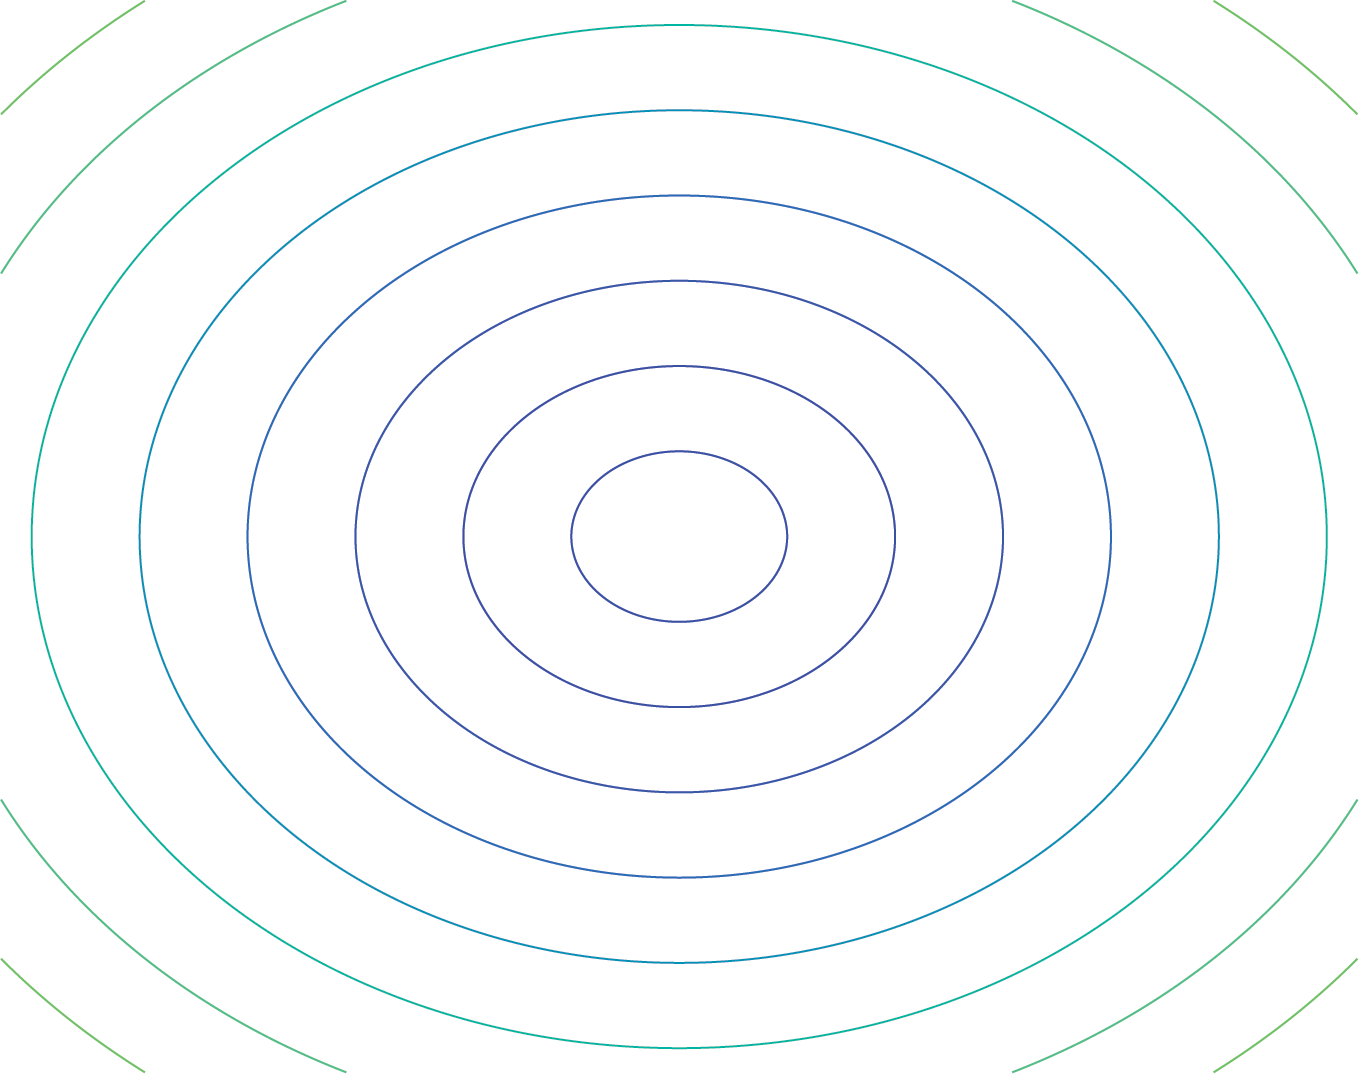
\includegraphics[width=\textwidth]{img/norm2}
		
		$\ell_2$
		\end{center}
		\end{minipage}\hfill
		\begin{minipage}{.3\textwidth}
		\begin{center}
		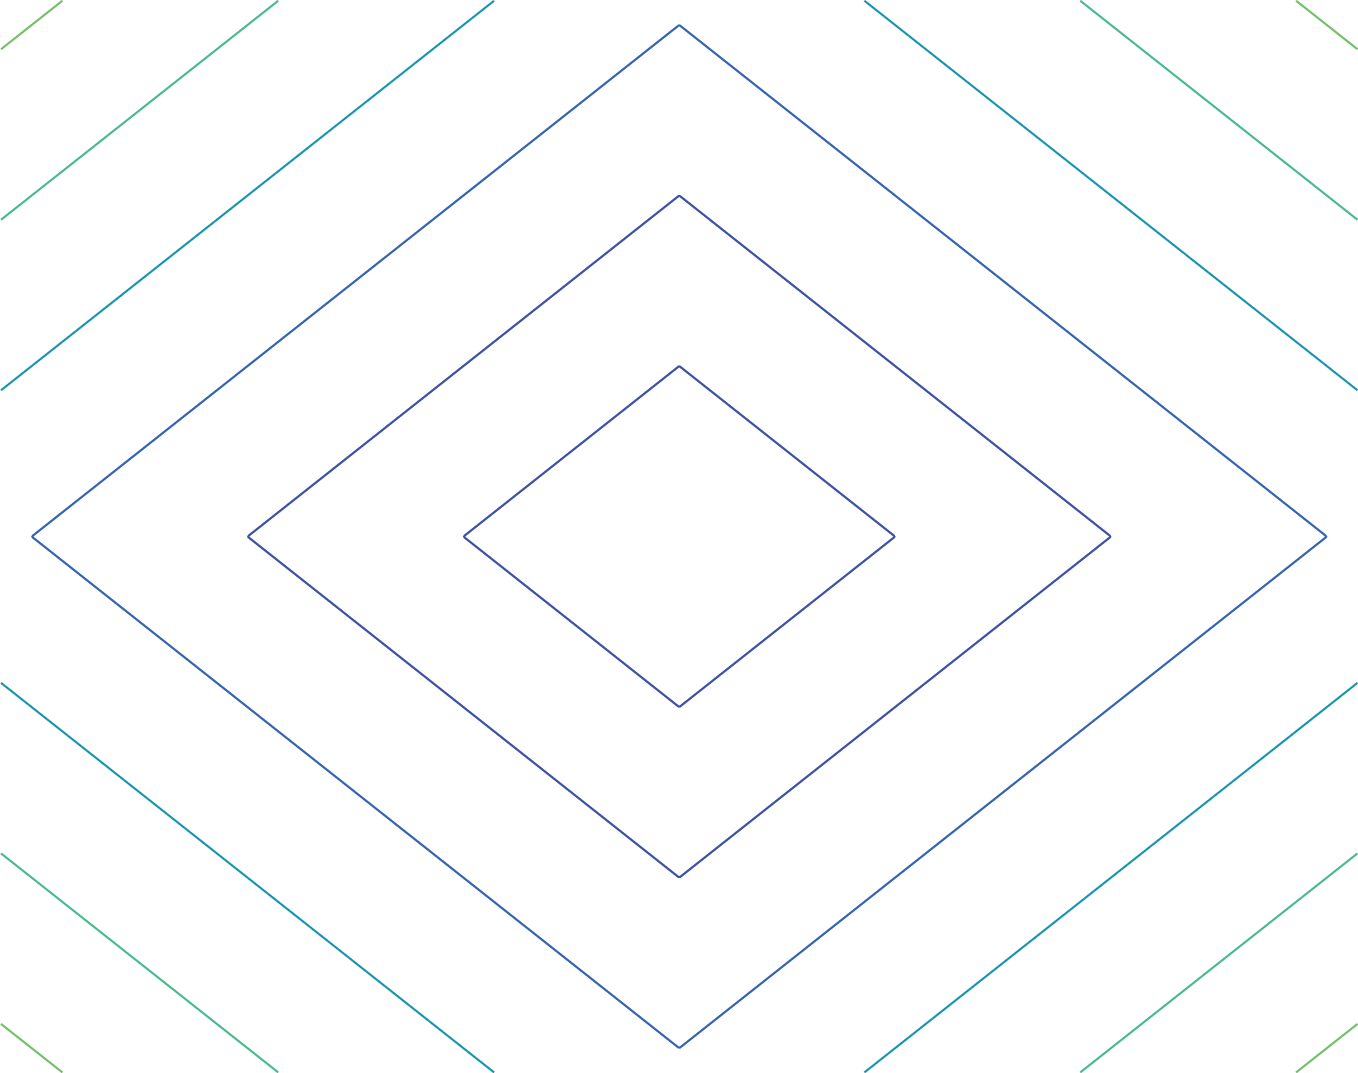
\includegraphics[width=\textwidth]{img/norm1}
		
		$\ell_1$
		\end{center}
		\end{minipage}\hfill
		\begin{minipage}{.3\textwidth}
		\begin{center}
		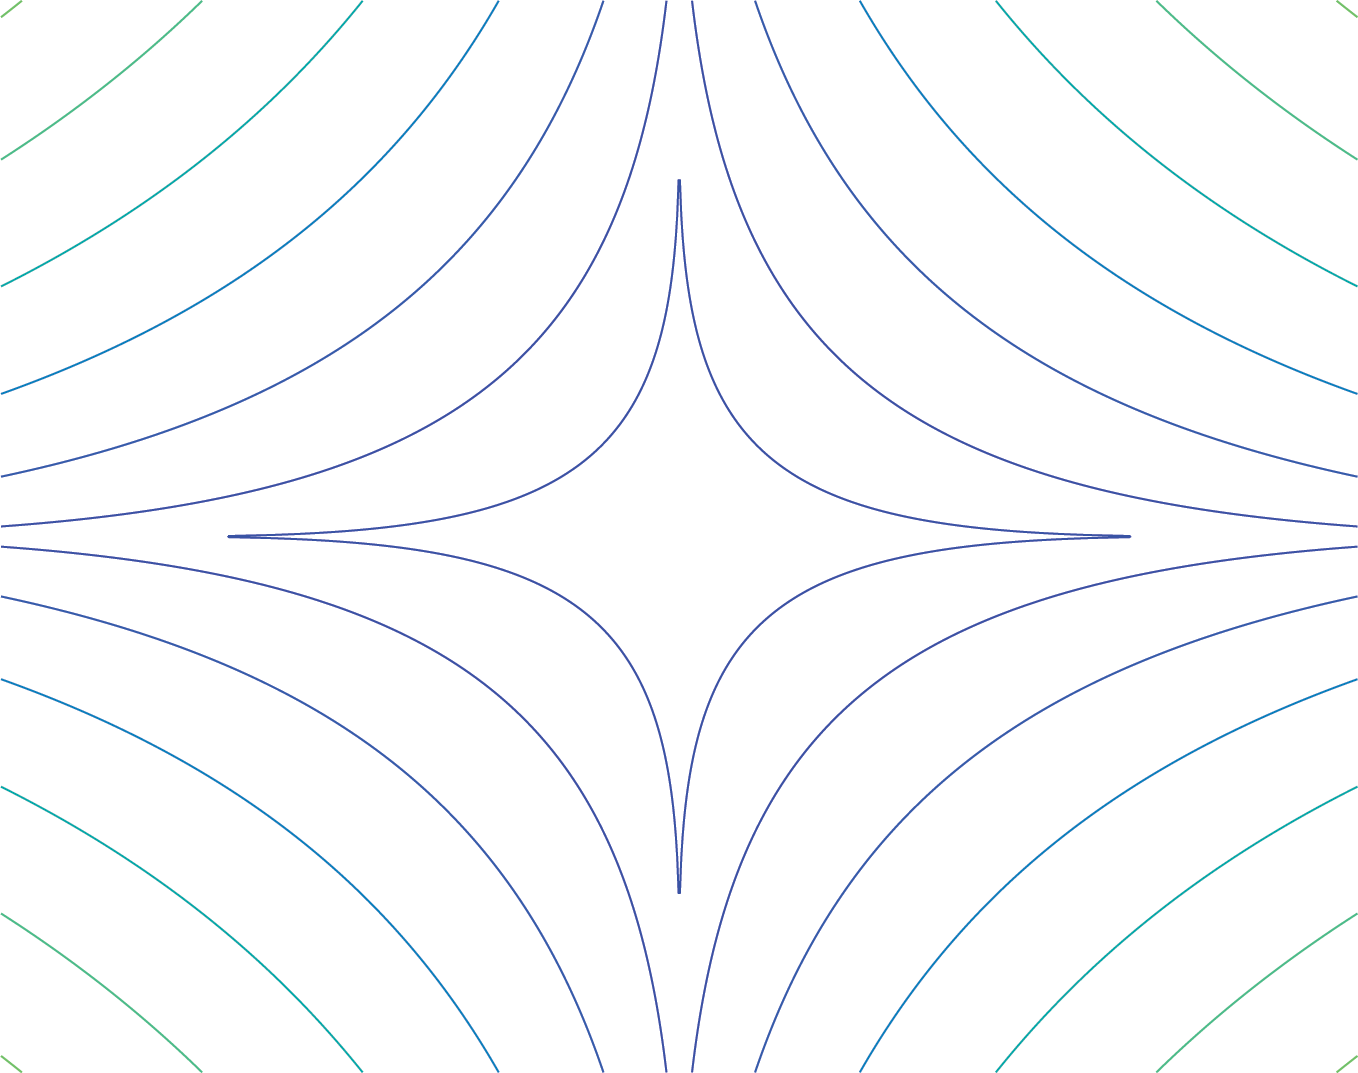
\includegraphics[width=\textwidth]{img/norm04}
		
		$\ell_{0.4}$
		\end{center}
		\end{minipage}

		\end{center}
		\end{frame}
		
		
		\begin{frame}
		\frametitle{Sparse recovery}
		\begin{center}
		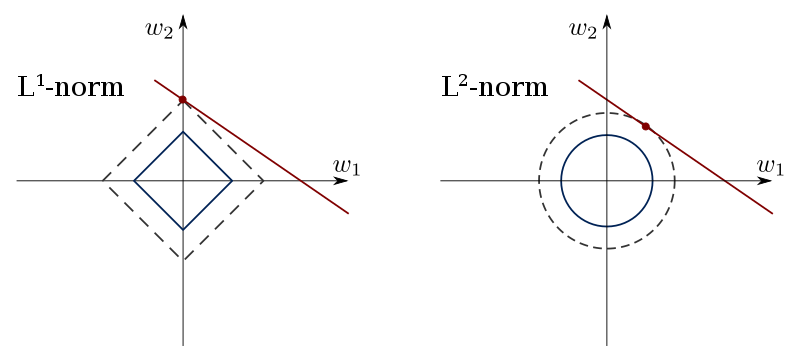
\includegraphics[width=.8\textwidth]{img/l1l2}
		\end{center}
		\end{frame}

		\begin{frame}
		\frametitle{Sparse recovery (Lasso)}
		\begin{equation}
		\nonumber x^* = \argmin_{x\in \rd}\onehalf\normtwosq{Ax-y} + \lambda\norm{x}_1
		\end{equation}

		\quad \\ \quad \\ \quad \\
		\begin{equation}
		\nonumber
		x^* = \argmin_{x\in \rd}\norm{x}_1\qquad \text{ s.t. } \normtwosq{Ax-y}\le\varepsilon
		\end{equation}
		\end{frame}
		
		\begin{frame}
		\frametitle{$\Prox$ of norms}
		Consider $g = \norm{\cdot}$ and $\mathcal{B} = \left\{x : \norm{x}_*\le 1 \right\}$, then
		\begin{equation}
		\nonumber g^* \left(\xi\right) = \iota_\mathcal{B}\left(\xi\right)
		\end{equation}
		
		By Moreau decomposition:
		\begin{gather}
		\nonumber v = \prox{\norm{\cdot}}{v} + \Pi_{\mathcal{B}}(v)\\
		\nonumber \prox{\norm{\cdot}}{v} = v - \Pi_{\mathcal{B}}(v)
		\end{gather}
		\pause
		\begin{center}
		\textbf{We have the proximal operator of norms!}
		\quad \\ \quad \\
		
		Sparse recovery can be solved
		\end{center}
		\end{frame}
		
		\begin{frame}
		\frametitle{Structured sparsity}
		Necessity to \emph{exclude} blocks of $x$
		
		\begin{itemize}
		\item Non-Overlapping Group Lasso
		\item Overlapping Group Lasso
		\item Hierarchical Lasso
		\end{itemize}
		\end{frame}
		
		\begin{frame}
		\frametitle{Non Overlapping Group Lasso}
		\begin{equation}
		\nonumber \Omega(x) = \norm{X_\mathcal{G}}_1 = \sum_{g\in\mathcal{G}} w_g \norm{x_{|g}}_2
		\end{equation}
		\pause
		
		By separability of $\Prox$ we have
		
		\begin{equation}
		\nonumber \prox{\Omega}{x} = \prox{g_1}{\prox{g_2}{\dots\prox{g_k}{x}}}
		\end{equation}
		\end{frame}
		
		\begin{frame}
		\frametitle{Overlapping Group Lasso}
		\begin{equation}
		\nonumber \Omega(x) = \sum_{g\in\mathcal{G}} w_g \norm{x_{|g}}_2
		\end{equation}
		\pause
		
		Much more complicated \pause but feasible		
		\end{frame}
		
		\begin{frame}
		\frametitle{Hierarchical Sparsity}
		\begin{center}
		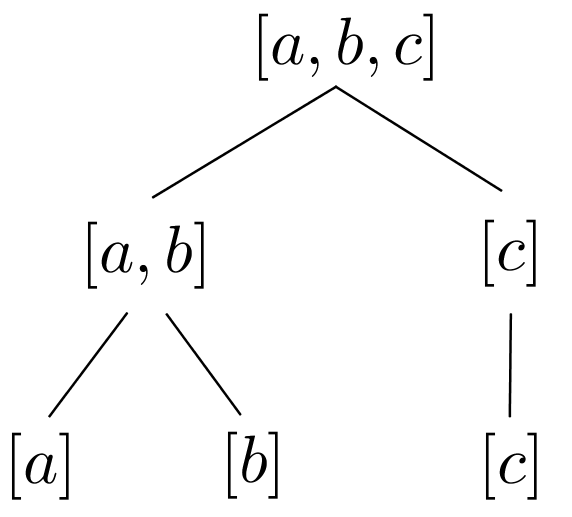
\includegraphics[width=.3\textwidth]{img/treestructuretransparent.png}
		
		\begin{equation}
		\nonumber \prox{\Omega}{x} = \prox{g_1}{\prox{g_2}{\dots\prox{g_k}{x}}}
		\end{equation}
		\end{center}
		\end{frame}
		
		\begin{frame}
		\frametitle{Proximal of Hierarchical Sparsity}
		Let $(\mathcal{G}, \preceq)$ be ad ordered tree structure
		\begin{enumerate}
		\item Set $v = x$.
		\item For $g\in\mathcal{G}$ following $\preceq$ do
		\begin{equation}
		\nonumber
		v_{|g} \longleftarrow v_{|g} - \Pi_{\norm{\cdot}_*\le\omega_g}\left(v_{|g}\right).
		\end{equation}
		\end{enumerate}
%		\quad \\ \quad \\ \quad \\ \quad \\
%		{\footnotesize Jenatton et al., ``Proximal methods for sparse hierarchical sparse dictionary learning'', 2010}
		\end{frame}
		
		
		\begin{frame}
		\frametitle{Non-Negativity constraint}
		\quad \\ \quad \\
		
		\begin{equation}
		\nonumber x^* = \argmin_{x\in\rd} \underbrace{f(x)}_{\text{s}} + \underbrace{g(x) + \iota_{\ge 0}(x)}_{\text{ns}}
		\end{equation}
		
		\pause
		\begin{definition}[Absolute norm]
		A norm $\Omega: X\to \RR$ is called \emph{absolute} if $\forall u,v\in\RR^N$ such that $|u_j|\le |v_j|$ for all $j$ implies $\Omega(u)\le \Omega(v)$.
		\end{definition}
		
		\begin{theorem}[Proximal operator of absolute norms]
		Let $w\in\RR^n$ and $\lambda>0$. Consider an absolute norm $\Omega$. We have
		\begin{equation}
		\nonumber
		\argmin_{z\in\RR^n}\left[\frac{1}{2}\normtwosq{[w]_+ - z} + \lambda \Omega(z)\right] = \argmin_{z\in\RR^n_+}\left[\frac{1}{2}\normtwosq{w - z} + \lambda \Omega(z)\right].
		\end{equation}
		\end{theorem}
		\begin{equation}
		\nonumber
		\prox{\lambda\Omega}{[w]_+}  = \prox{\lambda\Omega+\iota_{\ge 0}}{w}
		\end{equation}
		\end{frame}
		
		
		\begin{frame}
		\frametitle{Sum up...}
		\begin{itemize}
		\item We can recover sparse variables/signals/codes/...
		\item Intrinsic structures can be exploited
		\item Proximal methods are the correct tools for sparse reconstruction
		\item Non-Negativity constraint can be embedded almost for free
		\end{itemize}
		\end{frame}
		
		\section{Brain Imaging}
		
		\begin{frame}
		\frametitle{Diffusion MRI}
		\quad \\ \quad \\
		\begin{center}
		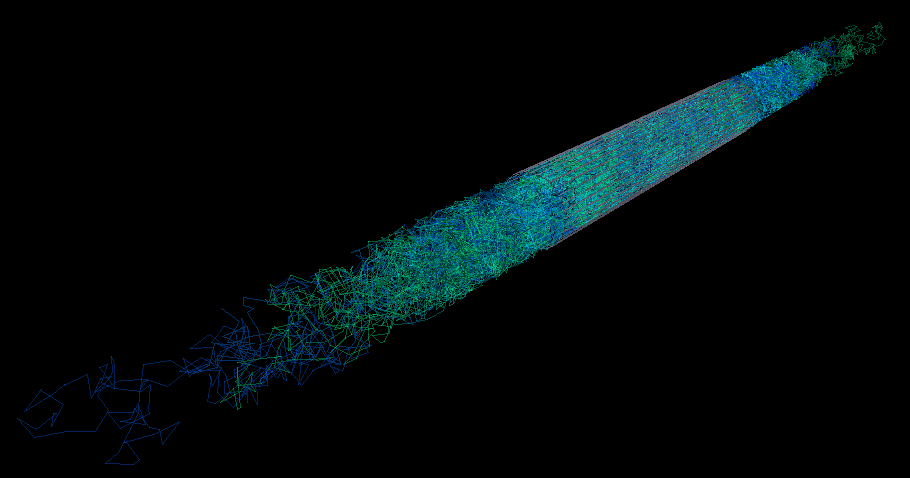
\includegraphics[width=.9\linewidth]{img/diffusion}
		\end{center}
		\end{frame}
		
		\begin{frame}
		\frametitle{Tractography}
		\quad \\ \quad \\
		\begin{center}
		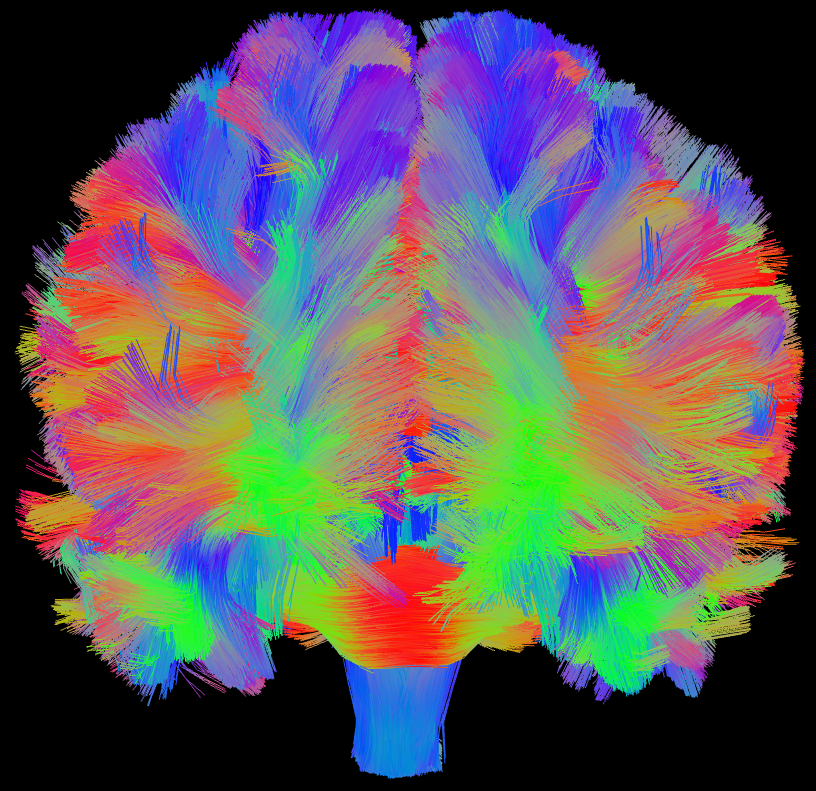
\includegraphics[width=.5\linewidth]{img/fulltract}
		\end{center}
		\end{frame}
		
		\begin{frame}
		\frametitle{Brain hierarchy}
		\quad \\
		
		\begin{minipage}{.4\linewidth}
		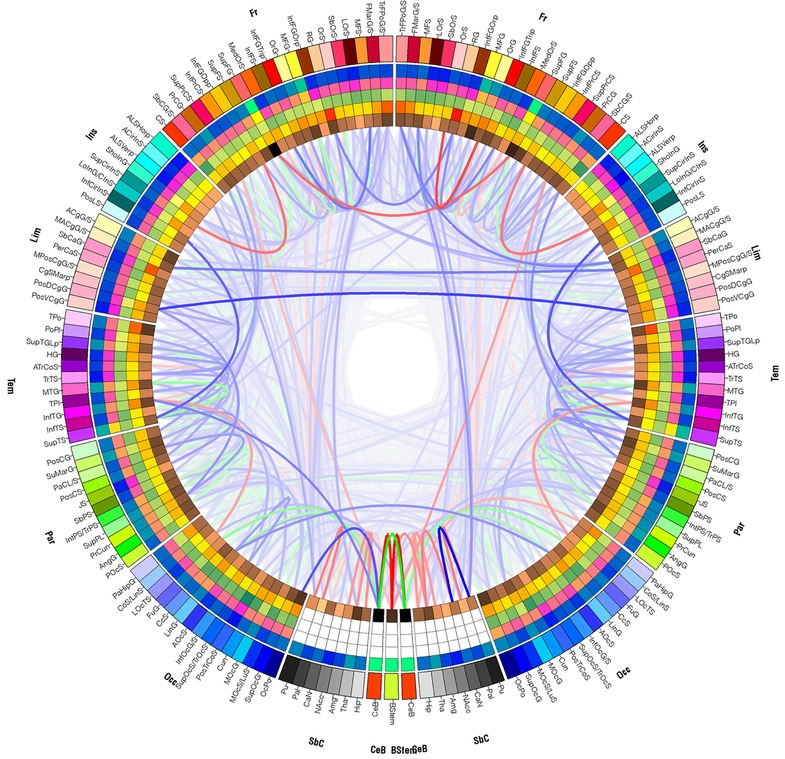
\includegraphics[width=\textwidth]{img/connectogram_transparent}\\
		\end{minipage}\hfill
		\begin{minipage}{.4\linewidth}
		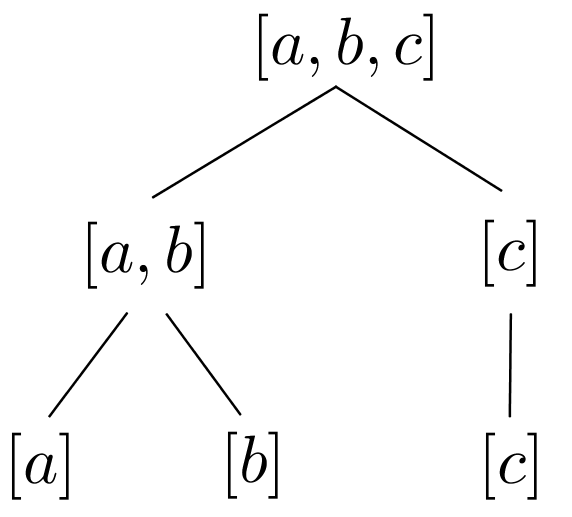
\includegraphics[width=\textwidth]{img/treestructuretransparent}
		\end{minipage}
		\end{frame}
		
		\begin{frame}
		\frametitle{The problem: false positives}
		\begin{center}
		\textbf{The challenge of mapping the human connectome based on diffusion tractography}
		\end{center}
		\begin{flushright}
		\emph{Maier-Hein et al., 2017 (Nature)}
		\end{flushright}
		
		\begin{itemize}
		\item 96 distinct tractography pipelines
		\item \emph{``most algorithms routinely extracted many false positive bundles''}
		\item \emph{``Tractography identifies more invalid than valid bundles''}
		\item \textbf{``Tractography is fundamentally ill‐posed''}
		\end{itemize}
		\end{frame}
		
		\begin{frame}
		\frametitle{Forward model: COMMIT}
		\quad \\ \quad \\
		\begin{center}
		\begin{minipage}{.15\linewidth}
		\begin{center}
		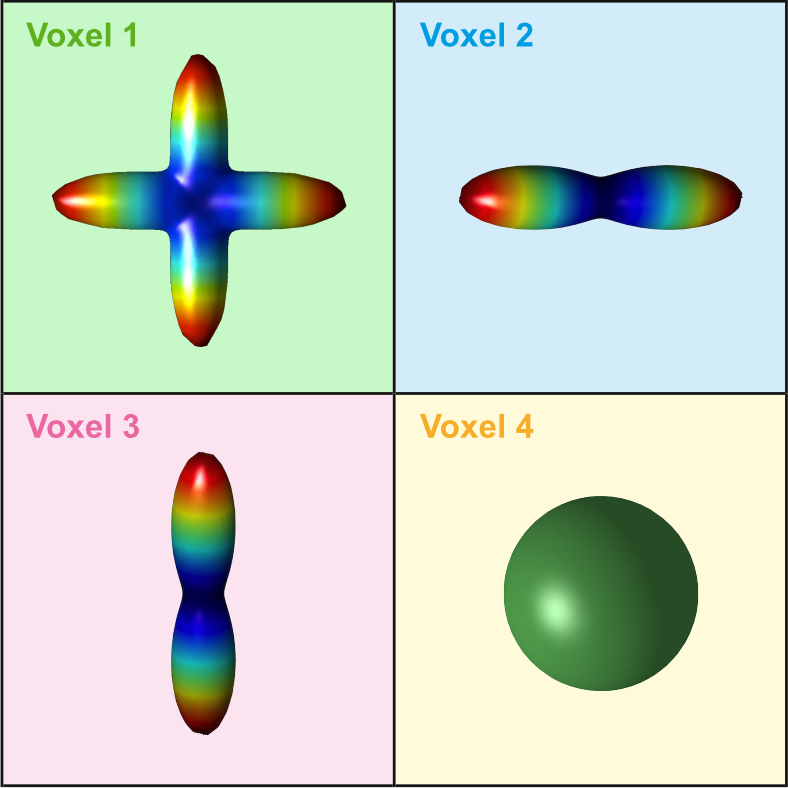
\includegraphics[width=\linewidth]{img/commit/COMMIT_idea_1_var}
		\end{center}
		\end{minipage}\qquad \qquad
		\begin{minipage}{.15\linewidth}
		\begin{center}
		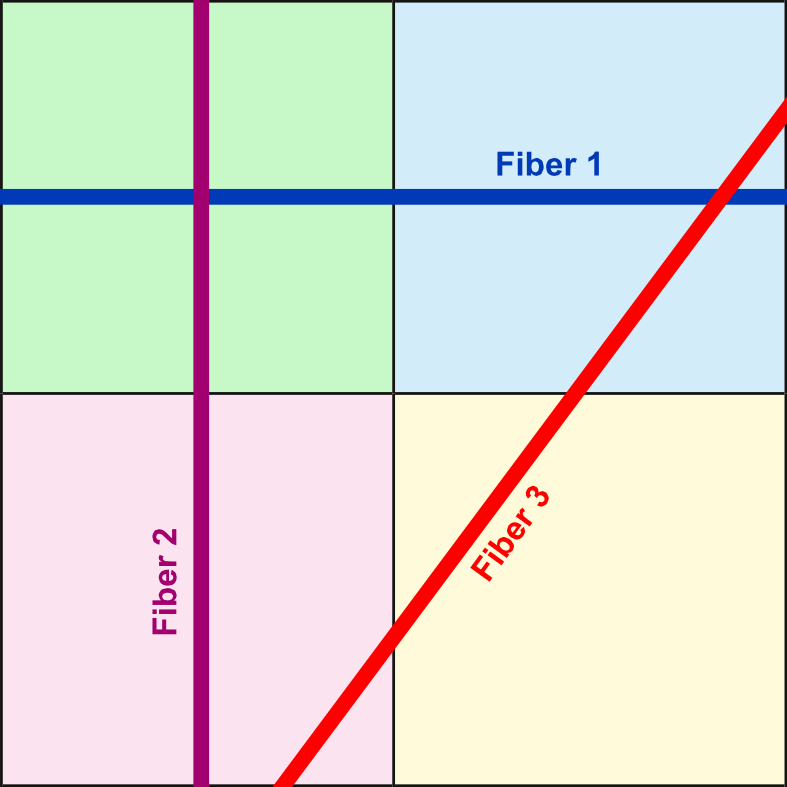
\includegraphics[width=\linewidth]{img/commit/COMMIT_idea_2_var}
		\end{center}
		\end{minipage}
		
		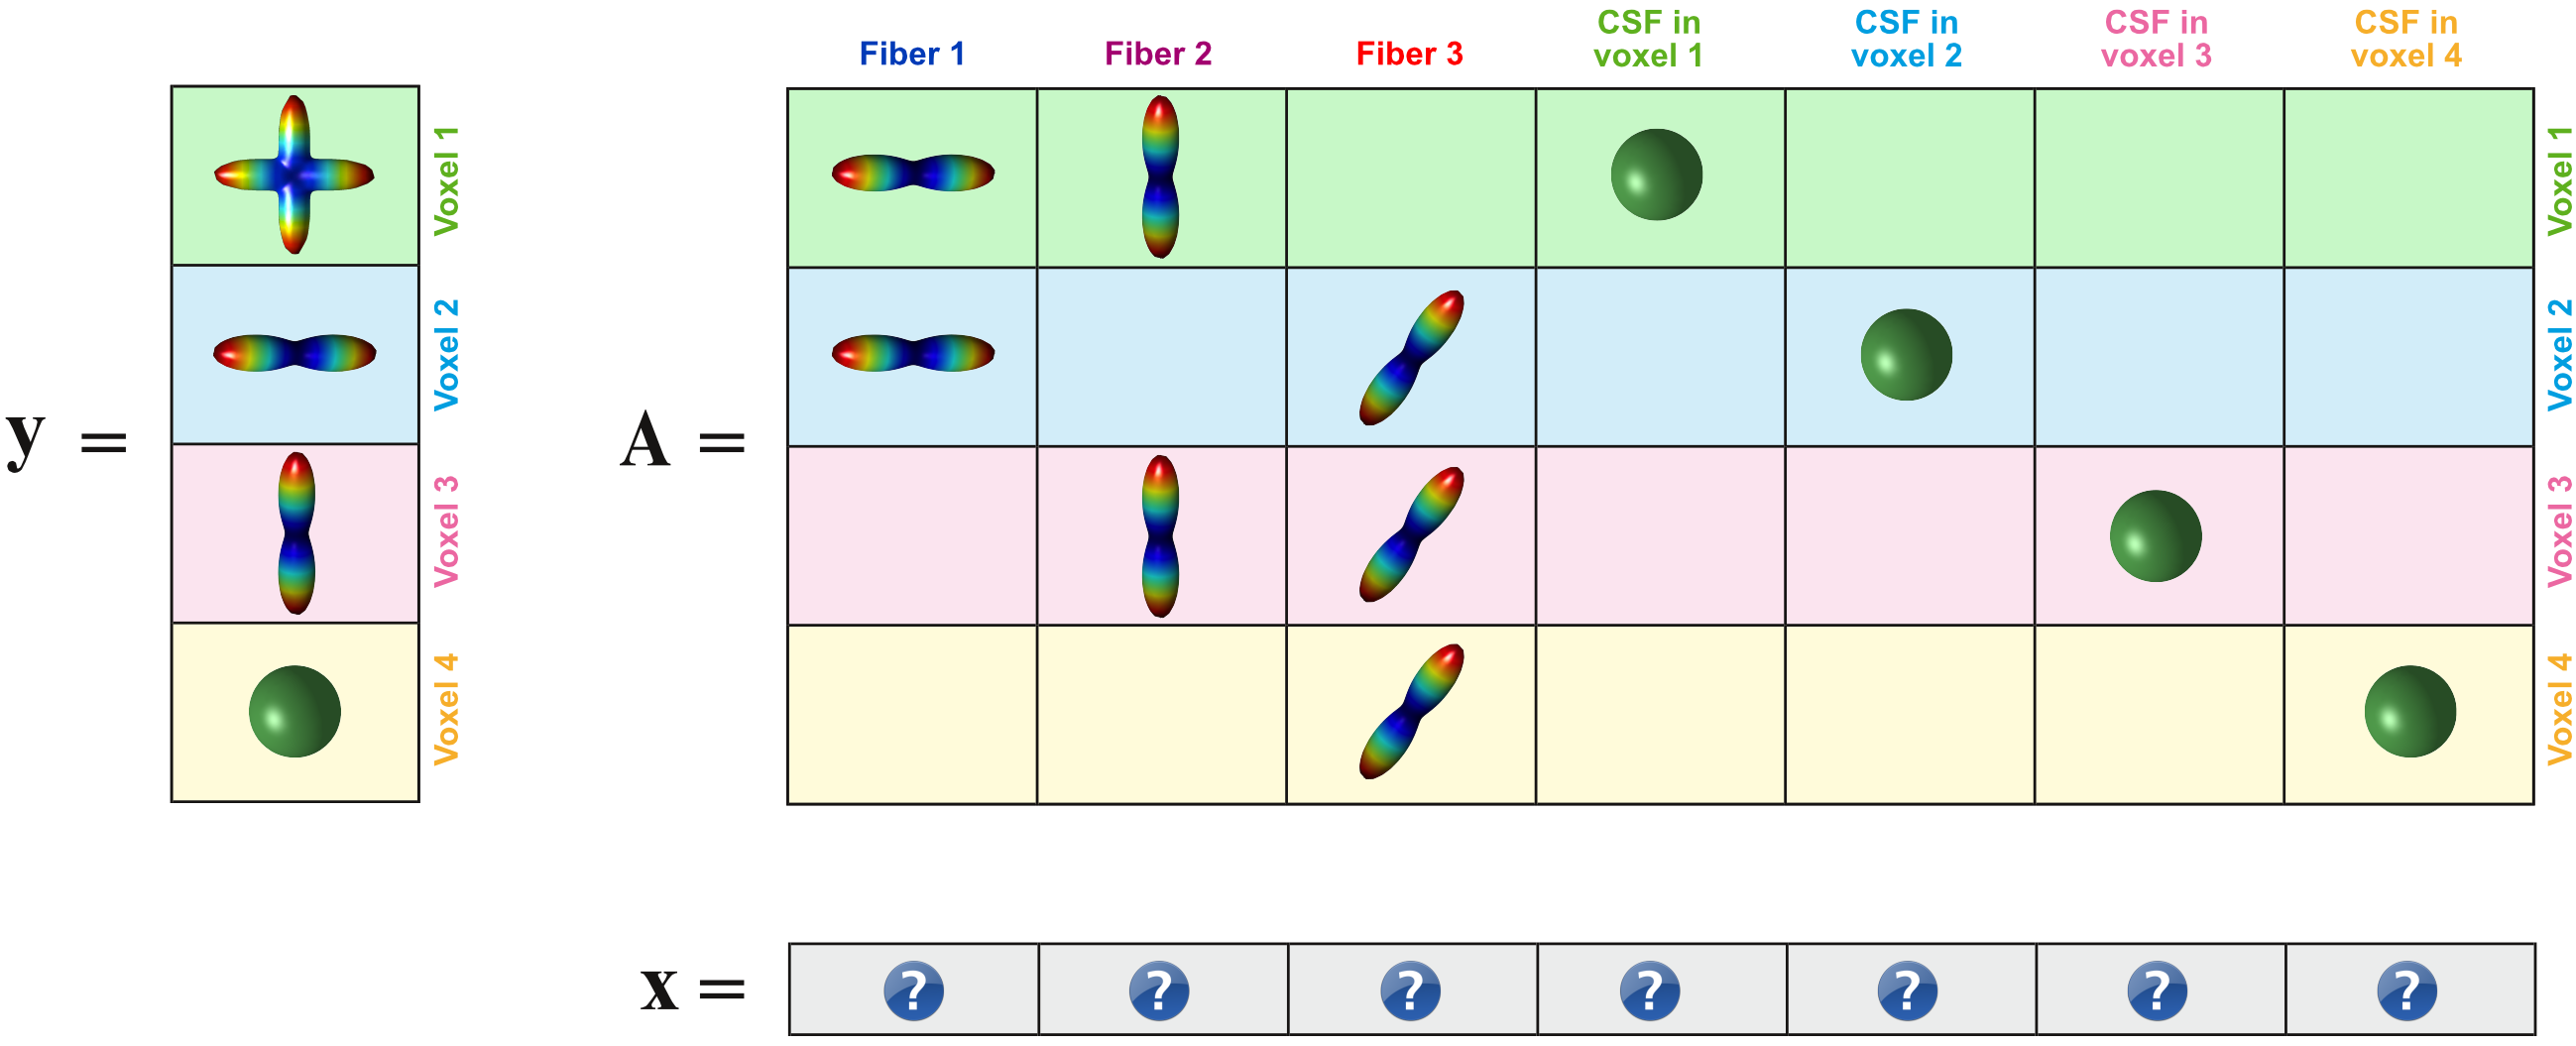
\includegraphics[width=.8\linewidth]{img/commit/COMMIT_idea_7}
		\end{center}
		\end{frame}
		
		\begin{frame}
		\frametitle{Forward model: COMMIT}
		\quad \\ \quad \\
		\begin{center}
		\begin{minipage}{.15\linewidth}
		\begin{center}
		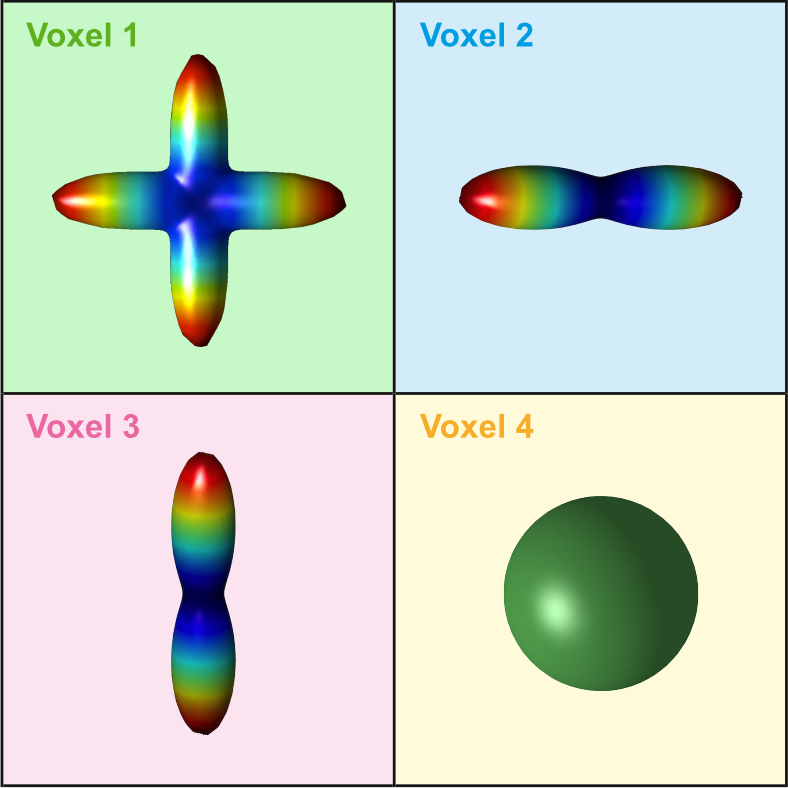
\includegraphics[width=\linewidth]{img/commit/COMMIT_idea_1_var}
		\end{center}
		\end{minipage}\qquad \qquad
		\begin{minipage}{.15\linewidth}
		\begin{center}
		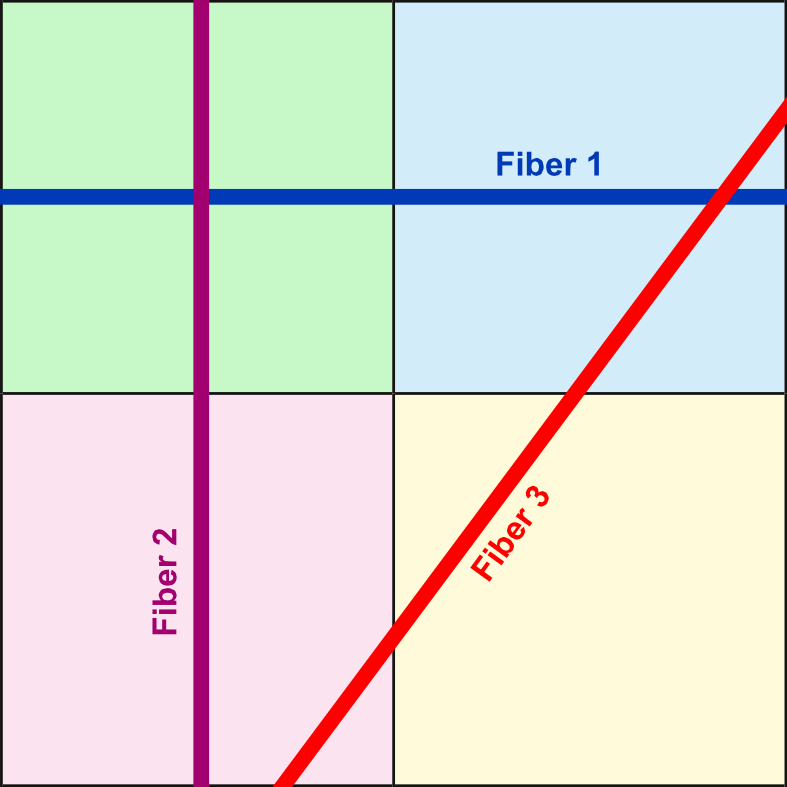
\includegraphics[width=\linewidth]{img/commit/COMMIT_idea_2_var}
		\end{center}
		\end{minipage}
		
		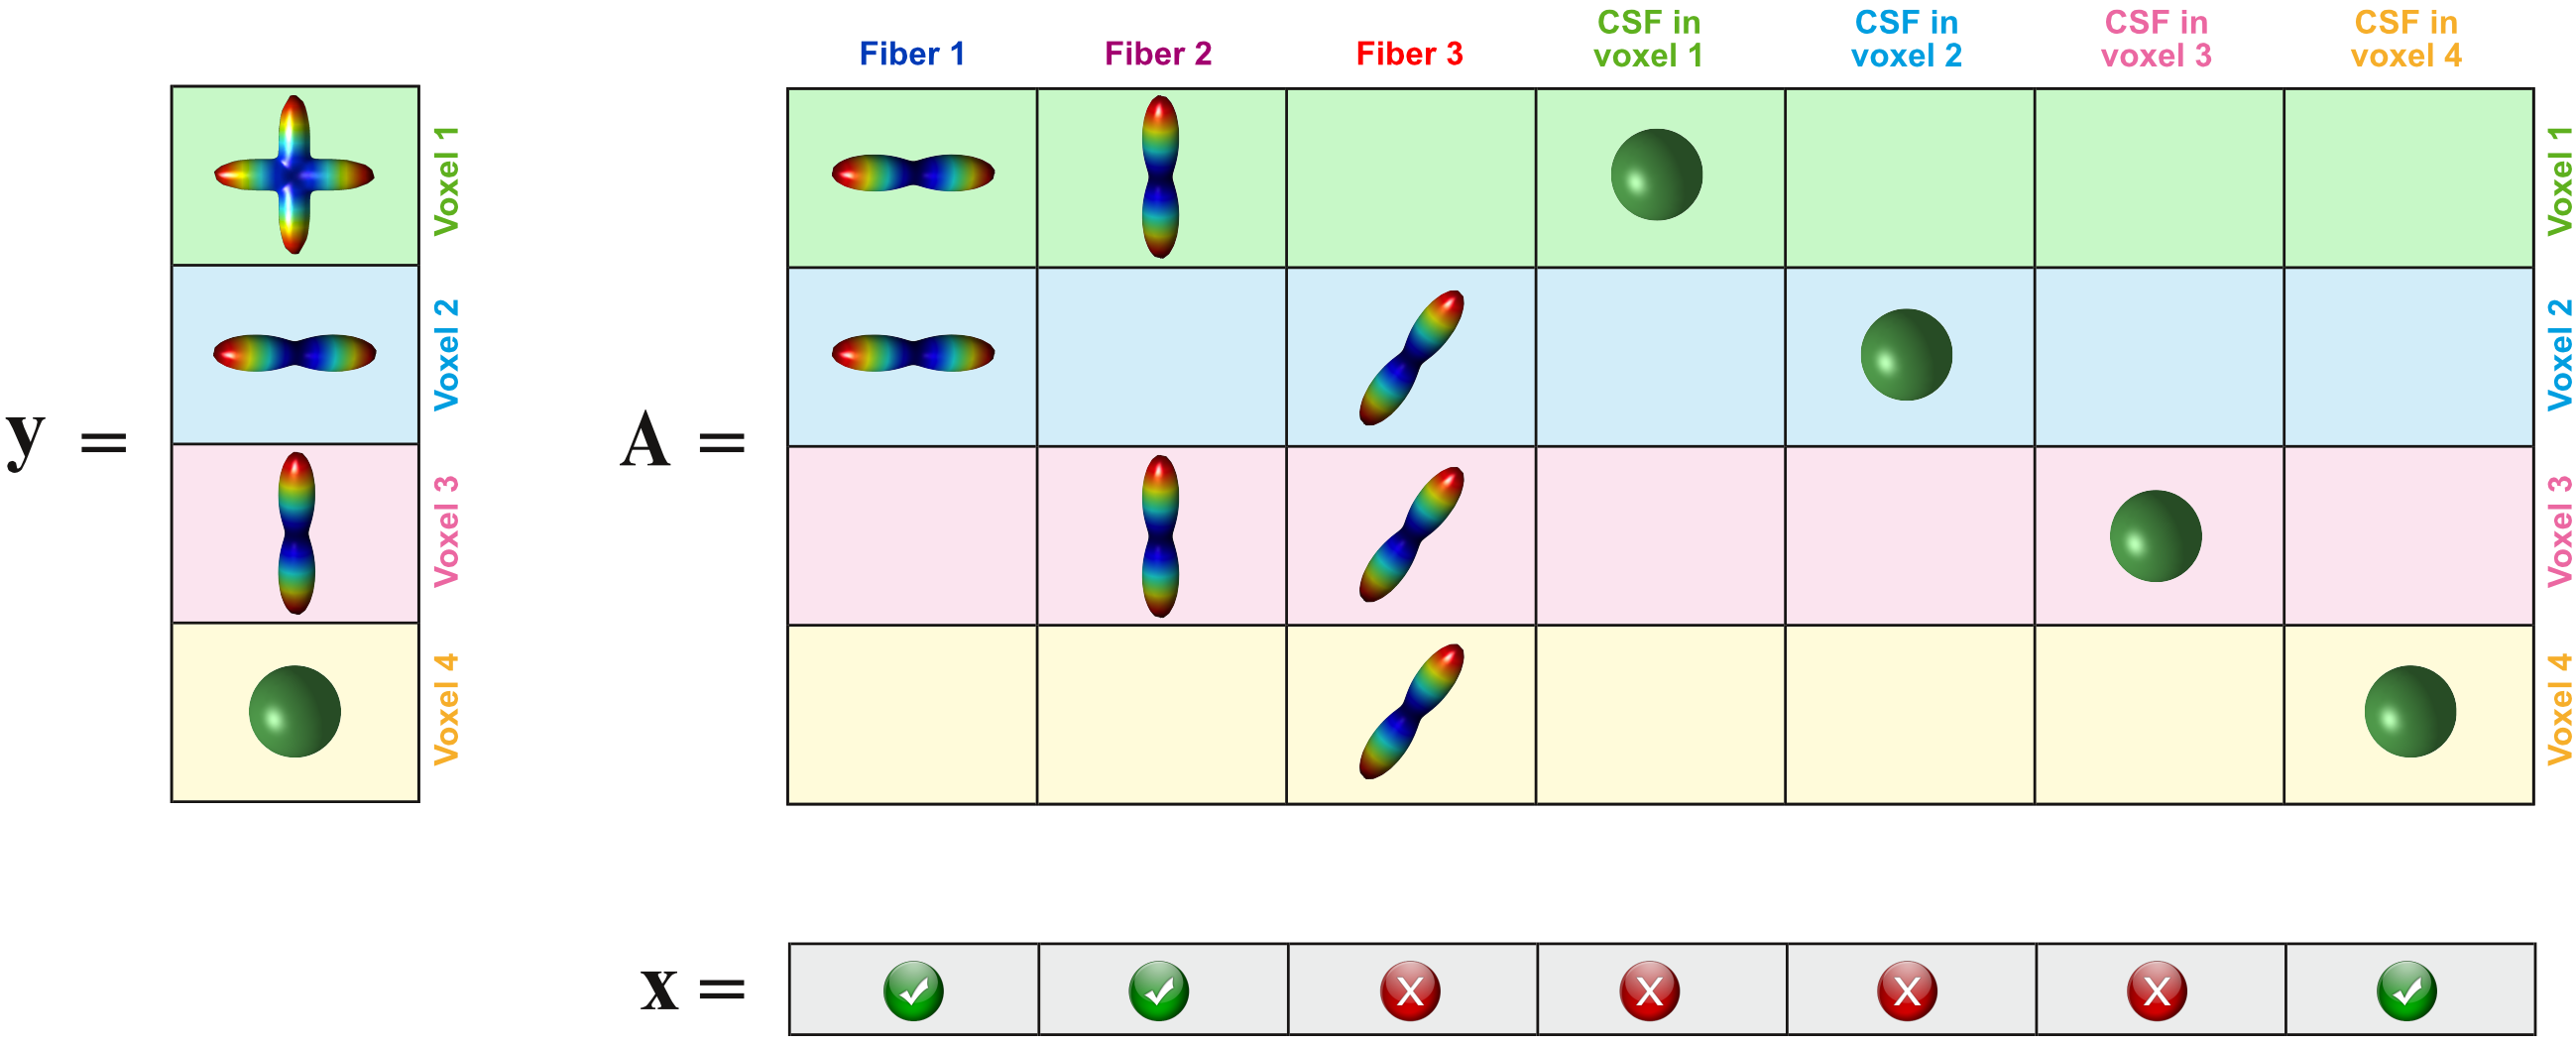
\includegraphics[width=.8\linewidth]{img/commit/COMMIT_idea_8}
		\end{center}
		\end{frame}
		
		\begin{frame}
		\frametitle{Hierarchical pattern}
		\begin{minipage}{.25\textwidth}
		\quad \\
		\quad \\
		\quad \\
		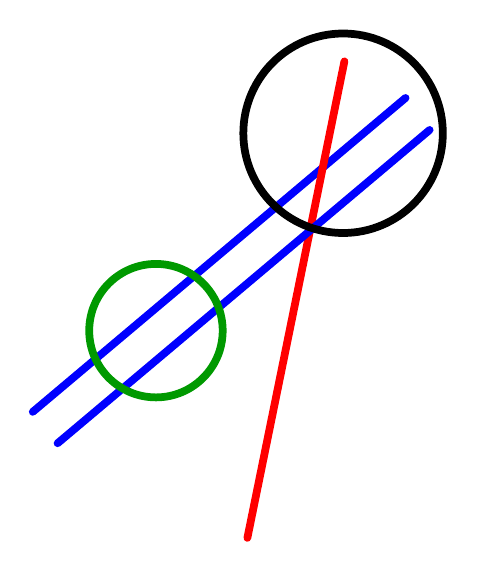
\begin{tikzpicture}[line cap=round,line join=round,>=triangle 45,x=1.0cm,y=1.0cm]
		\clip(2.4,0.75) rectangle (7.75,7.3);
		\draw [line width=2.8pt,color=qqqqff] (2.4644395930954643,2.4205807099751278)-- (7.199120666518885,6.4076805612790615);
		\draw [line width=2.8pt,color=ffqqqq] (6.422554452918324,6.872100757665542)-- (5.190243033337279,0.8200824526119717);
		\draw [line width=2.8pt,color=qqqqff] (2.7798456657281436,2.0219752974552785)-- (7.504966362216294,6.001024305024248);
		\draw [line width=2.8pt] (6.405604560046194,5.959117174062875) circle (1.2667403722174913cm);
		\draw [line width=2.8pt,color=qqzzqq] (4.0290654383489075,3.4521255090473444) circle (0.847551919863971cm);
		%\draw [line width=2.8pt,color=qqzzqq] (5.553853552823379,2.385862623546985) circle (0.5538395445164014cm);
		\end{tikzpicture}
		\end{minipage}\hfill
		\begin{minipage}{.5\textwidth}
		\begin{center}
		\quad \\
		\quad \\
		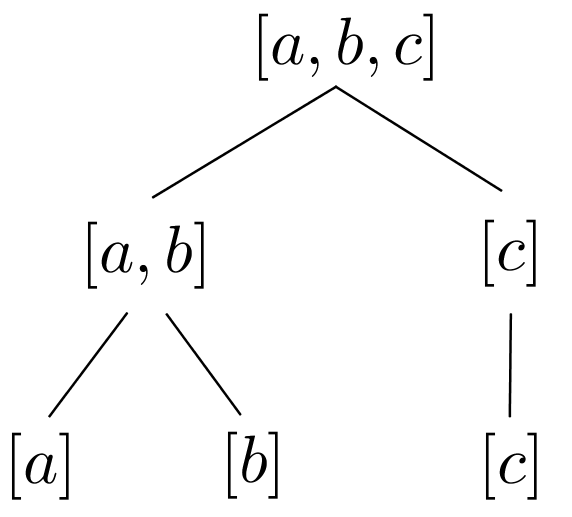
\includegraphics[width=.7\textwidth]{img/treestructuretransparent}
		\begin{equation}
		\nonumber \mathcal{G} = \Bigl(\bigl[{\color{blue}[a]},{\color{blue}[b]},{\color{mygreen}[a,b]},{\color{red}[c]},[a,b,c]\bigr],\preceq\Bigr)
		\end{equation}
		\end{center}
		{\flushleft NB:}
		\begin{equation}
		\nonumber [a]\preceq [a,b] \preceq [c] \qquad \nonumber [a,b,c]\npreceq [c]
		\end{equation}
		\end{minipage}
		\end{frame}
		
		\begin{frame}
		\frametitle{False positives detection}
		\begin{itemize}
		\item Build the dictionary/matrix $A$
		\item Fit the acquired dMRI signal
		\item Force hierarchical sparsity
		\pause\item \textbf{Impose non-negativity of $x$}
		\end{itemize}
		
		\pause
		
		\begin{equation}
		\nonumber x^* = \argmin_{x\in \rd}\onehalf\normtwosq{Ax-y} + \lambda \sum_{g\in\mathcal{G}}w_g\norm{x_{|g}}_2 + \iota_{\ge 0}(x)
		\end{equation}
		\end{frame}
		
		\begin{frame}
		\frametitle{Results}
		\quad \\ \quad \\
		\begin{center}
		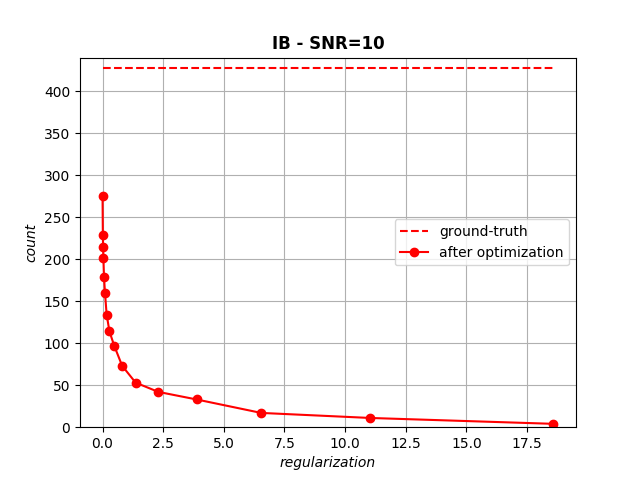
\includegraphics[width=.7\linewidth]{img/ResultsIBtr.png}
		\end{center}
		\end{frame}
		
		\begin{frame}
		\frametitle{Sum up...}
		\begin{itemize}
		\item Brain connections are organised with an hierarchical pattern
		\item False positives can be detected with structured sparsity
		\item The solution can be obtained via proximal splitting methods
		\pause\item It works :)
		\end{itemize}
		\quad \\ \quad \\ \quad \\ \quad \\
		\pause
		\begin{center}
		{\Huge \textbf{\smiley Thank you \smiley}}
		\end{center}
		\end{frame}
		
\end{document}